\documentclass[11pt,a4paper, openany]{memoir}
\usepackage[utf8]{inputenc}
\usepackage[T1]{fontenc}
\usepackage{times}
\usepackage[french]{babel}
\usepackage{titlesec} % For chapter formatting
\usepackage{tikz}
\usepackage{fancyhdr}
\usepackage{graphicx} % includegraphics
\graphicspath{ {images/} }
\usepackage[
breaklinks=true,colorlinks=true,
linkcolor=black,urlcolor=black,citecolor=black,
bookmarks=true,bookmarksopenlevel=2]{hyperref}  % Links color in pdf
\usepackage{bookmark} % Creates bookmarks in pdf files
\usepackage[
  top=2.5cm,
  bottom=2.5cm,
  left=2.5cm,
  right=2.5cm,
  headsep=3pt,
  footskip=30pt,
  headheight=46pt,
  asymmetric
]{geometry}

% Header
\pagestyle{fancy}
\fancypagestyle{main}{%
  \lhead{
\includegraphics[scale=0.5]{HEIG-VD}}
  \rhead{\sffamily Projet Réseau de Petri\\Bise Léonard\\Informatique Embarquée (ISEC)}
  \rfoot{Page \thepage}
  \cfoot{}
}
\fancypagestyle{plain}{%
  \lhead{
\includegraphics[scale=0.5]{HEIG-VD}}
  \rhead{\sffamily Projet Réseau de Petri\\Bise Léonard\\Informatique Embarquée (ISEC)}
    \rfoot{Page \thepage}
      \cfoot{}
}

% Modifie la section chapitre
\titleformat{\chapter}
  {\sffamily\LARGE\bfseries}{\thechapter}{1em}{}
% spacing: how to read {12pt plus 4pt minus 2pt}
%           12pt is what we would like the spacing to be
%           plus 4pt means that TeX can stretch it by at most 4pt
%           minus 2pt means that TeX can shrink it by at most 2pt
%       This is one example of the concept of, 'glue', in TeX
\titlespacing*{\chapter}{0pt}{3.5ex plus 1ex minus .2ex}{2.3ex plus .2ex}
% Sets sections to sans serif
\setsecheadstyle{\LARGE\bfseries\sffamily}
\setsubsecheadstyle{\Large\bfseries\sffamily}
\setsubsubsecheadstyle{\large\bfseries\sffamily}
\setparaheadstyle{\large\bfseries\sffamily}
\setsubparaheadstyle{\large\bfseries\sffamily}

\begin{document}

%%%%%%%%%%%%%%%%%%%%% Page de Titre %%%%%%%%%%%%%%%%%%%%%%

\thispagestyle{empty}

\sffamily

% Logo HEIG-VD
\begin{tikzpicture}[remember picture,overlay]
\node[anchor=north west,yshift=-40pt,xshift=40pt]%
        at (current page.north west)
        {
\includegraphics[scale=0.8]{HEIG-VD}};
\end{tikzpicture}

\large

~\vspace{\fill}

\begin{center}
{\HUGE 
Gestion d'un carrefour à l'aide d'un réseau de Petri
}
\vspace{1cm}
\hrule
\vspace{1cm}
{\LARGE
Rapport du projet
}
\end{center}

\vspace{3.5cm}

\begin{flushleft}
Auteur: Bise Léonard\\
Professeur: Zysman Eytan\\
Filière: Informatique Embarquée (ISEC)\\
Cours: Programmation Concurrente (PConc)\\
Date: 10 Mai 2018
\end{flushleft}

\vspace{\fill}

\cleardoublepage

%%%%%%%%%%%%%%%%%%%%%% Table des matières %%%%%%%%%%%%%%%%%%%%%%%

\tableofcontents

\clearpage

%%%%%%%%%%%%%%%%%%%%%% Liste des figures %%%%%%%%%%%%%%%%%%%%%%%

%\listoffigures  % Write out the List of Figures

%\clearpage

%%%%%%%%%%%%%%%%%%%%%% Liste des Tables %%%%%%%%%%%%%%%%%%%%%%%

%\listoftables  % Write out the List of Tables

%\clearpage

%%%%%%%%%%%%%%%%%%%%%% Introduction %%%%%%%%%%%%%%%%%%%%%%%

\chapter{Introduction}

Dans le cadre du cours Programmation Concurrente (PConc), il nous a été demandé de créer un programme qui simule le comportement d'un carrefour. Le carrefour est composé de deux flux, un Sud-Nord et l'autre Ouest-Est ou les voitures circulent dans un seul sens. A l'intersection des deux flux sont placé deux feux de signalisation, un par flux, ils permettent ou non au voiture de passer.\par
La gestion du système est fait grâce à un réseau de Petri qui réagit aux événement et qui produit des actions.

\chapter{Cahier des Charges}

Dans le cadre du projet il nous est demandé de créer un projet codé en java comprenant les éléments suivants:
\begin{itemize}
\item Créer un gestionnaire de réseau de petri auquel il est possible de donner un fichier de configuration pour créer un paysage (création des places, transition, arcs de pre et post incidence).
\item Lorsque le réseau de Petri est créé, il est possible de lancer la simulation, à chaque tick le gestionnaire va faire évoluer le réseau de Petri en regardant quelle places sont sensibilisée, il va ensuite consommer et produire des jetons aux places requises.
\item Lorsqu'un jeton arrive dans une place, si l'utilisateur a lié une action à la place, le gestionnaire va lancer l'exécution de l'action
\item L'environnement éxtérieur doit pouvoir ajouter des événements dans une queue, ce qui permettra aux transitions d'être franchies lorsqu'elles sont sensibilisées.
\item Utiliser le gestionnaire de réseau de Pétri afin d'implémenter un réseau qui permet la gestion d'un carrefour avec deux flux perpendiculaire de voiture et qui est à sens unique. Il existe deux réseau de Petri qui sont décrit dans les slides de Monsieur Zysman, un avec timer intégré et l'autre sans. Pour ce projet le plus simple des deux sera utilisé, c'est à dire sans timer intégré. Le réseau de Petri est défini avec détail dans les slides à la page 8.\\
\end{itemize}
En utilisant le gestionnaire de réseau de Petri, il faudra créer les éléments suivants et les faire intéragir avec le réseau pour faire évoluer le système.

\begin{itemize}
\item Un objet responsable de la gestion des deux routes, il permettra aux véhicules de savoir s'ils peuvent avancer ou si un véhicule se trouve déjà dans la case devant eux. La gestion se fait grâce à deux vecteurs un par flux, le croisement est donc présent dans chacun des deux flux
\item Deux threads, un par flux, qui crééront à des temps aléatoire de nouveaux véhicules, ils seront créés au début de la route
\item Un objet véhicule, cet objet, dès sa création, commencera à avancer de case en case en direction de la fin de la route. Lorsqu'il arrivera juste devant le carrefour il vérifiera si le feu est vert avant de pouvoir entrer dans le carrefour. Lorsqu'il atteint la fin de la route il disparait
\item Deux détecteurs, un par flux, qui auront comme tâche de déclencher un événement lorsqu'ils détecteront un véhicule présent juste avant le croisement
\item Deux détecteurs, un par flux, qui auront comme tâche de déclencher un événement lorsqu'ils détecteront que le croisement est vide
\item Deux feu de signalisation, un par flux, qui autoriseront ou non les véhicule du flux à passer dans le croisement
\end{itemize}

\chapter{Architecture}

L'image suivante montre l'architecture générale de l'application.

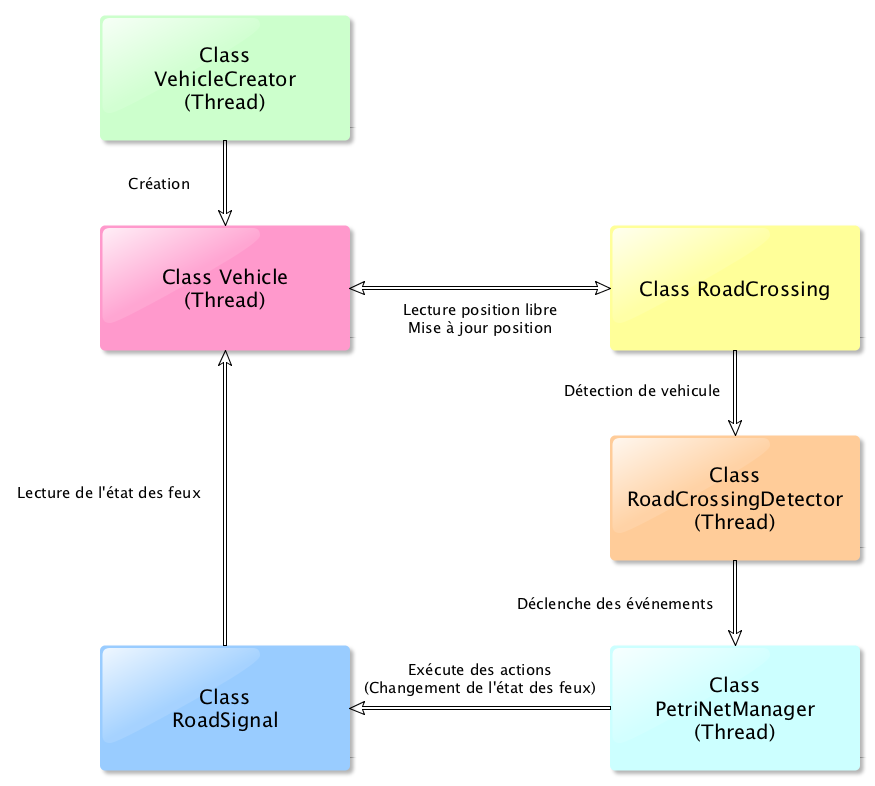
\includegraphics[scale=0.5]{images/architecture.png}

\chapter{Le mécanisme du Réseau de Petri}

La classe PetriNetManager implémente le gestionnaire de réseau de Petri. D'autres classes sont utilisées pour la gestion des réseaux, elles sont décrites ci-dessous.\\
\begin{itemize}
\item PetriNetManagerTest: Contient quelques tests du bon fonctionnement du gestionnaire de réseau
\item PetriArc: Décrit les caractèristiques lié aux arcs de pré et post incidence comme le type (simple, test, inhibit) et leur poids
\item PetriPlace: Une place dans un réseau de Petri ainsi que sont action liée si elle en as une
\item PetriPlaceInterface: Une interface qui permet à la classe qui l'implémente d'être ensuite déclenchée par le gestionnaire de réseau lorsqu'un jeton entre dans la place qui y est liée.
\item PetriTransition: Contient les informations relative à une transition faisant partie du réseau de Petri\\
\end{itemize}
La classe PetriNetManager est la classe centrale du gestionnaire de réseau de Petri. Après l'instanciation de la classe, un réseau de Petri peut être initialisé en utilisant la méthode loadFromTextFile avec un fichier de configuration. Ceci créera toute les places, transitions et arcs requis pour le réseau décrit.\\\\
Une fois le réseau initialisé l'utilisateur à la possibilité de faire les actions suivantes:
\begin{itemize}
\item Lier une place du réseau avec une classe implémentant l'interface PetriPlaceInterface avec la méthode setPlaceAction. Lorsque le gestionnaire du réseau détecte l'entrée d'un jeton dans la place, il déclenchera automatiquement l'exécution de l'action
\item Lancer le gestionnaire de réseau de Petri avec la méthode start. Cette action lancera l'exécution du Thread de PetriNetManager qui après chaque tick effectuera la simulation du réseau
\item Une fois le gestionnaire lancé, l'utilisateur doit déclencher des événements liés à une certaine transition au moyen de la méthode newEvent ce qui permettra le franchissement de la dite transition si elle est préalablement sensibilisée\\
\end{itemize}
Le coeur de la simulation du réseau de Petri est effectuée par la méthode step. Cette méthode simule un pas de  l'évolution du réseau de Petri, elle est cadencée par la durée d'un tick, c'est à dire un temps entre deux pas.\\
La liste suivante décrits les opérations effectuées par la méthode step, elle se découpe en quatre phases.\\
\begin{itemize}
\item Phase 0 : Les actions des places qui ont eu de nouveaux jetons sont appelées
\item Phase 1 : Le gestionnaire détermine les transitions qui sont sensibilisées, c'est à dire que les places qui y sont liées contiennent le nombre de jeton requis, et les ajoute dans une liste de transition sensibilisée. La liste est ensuite mélangée pour que les transitions aient un ordre aléatoire
\item Phase 2 : Pour chaque tranisition qui sont dans la liste des transitions sensibilisées, le gestionnaire vérifie si l'événment associé a été déclenché, c'est à dire si il est présent dans la queue d'événement. Si c'est le cas, les jetons des places qui sont liées à la transition sont consommés et elle est ajoutée à la liste des transitions franchies. La liste des transitions sensibilisées est à nouveau parcourue pour vérifier si certaines transitions ne le sont plus suite à la consommation de jetons
\item Phase 3: Les jetons nécessaire sont produit dans les places liées aux transitions qui ont été franchies
\end{itemize}

\chapter{Implémentation des acteurs}

Le projet de gestion de carrefour demande la création de différents acteurs qui sont listé ci-dessous.\\

\begin{itemize}
\item RoadCrossing: La grille sur laquelle les voitures se déplace. Cette classe est passive, elle ne fait que d'être modifié par d'autre classe, elle n'as pas son propre Thread. Les instance de Vehicle, l'utilise pour savoir si elles peuvent avancer ou si un autre véhicule se trouve déjà devant eux
\item RoadCrossingDetector: Les detecteurs utilisés pour déclencher des événements dans le réseau de Petri. Il y'en a deux par flux. Un placé juste avant le carrefour déclenchera l'événement lié à la détection de flux voulant entrer dans le carrefour, cela permet au réseau de Petri de faire passer le feu de l'autre flux au rouge et ainsi permettre au premier flux de pouvoir passer
\item RoadSignal: Le feu routier, c'est un élément passif qui ne fait que d'avoir un état, soit rouge ou alors vert. Il y a un feu par flux, les véhicules lorsqu'ils arrivent devant le carrefour doivent veiller à vérifier que le feu est vert avant de pouvoir y rentrer. L'état des feux est modifiés au travers de deux actions du réseau de Petri.
\item EventManager : C'est une classe qui permet de définir des événements réél et les associer a un événement du réseau de Petri en utilisant à l'interne des classes de type Event. C'est donc l'interface entre le monde réél et le réseau de Petri
\item RoadCrossingEventManager : Utilise la classe EventManager pour définir les événements qui sont propres au problème du carrefour (par exemple arrivée devant le carrefour ou sortie du carrefour)
\item SignalStateAction : Cette classe implémente l'interface PetriPlaceAction et défini donc l'action à effectuer lorsqu'un feu doit changer d'état. Elle directement appellé par le gestionnaire de réseau de Petri quand nécessaire et elle contient une réference au feu qu'elle doit gérer.
\item Vehicle : Définit le comportement d'un véhicule, après avoir été créé il commence à avancer régulièrement le long de son flux en utilisant la grille définie par la classe RoadCrossing. Juste avant de rentrer dans le carrefour la couleur du feu sera vérifiée pour voir si il est possible d'avancer. Lorsqu'elle arrive à la fin de la route, le véhicule a terminé sa vie et est détruit.
\item VehicleCreator : Ce Thread est responsable de la création de véhicule dans un certain flux de manière régulière
\item RoadSignalTimerAction : Cette classe représente l'action a effectuer lorsqu'un véhicule arrive devant le carrefour et que sont feu est rouge. Dans ce cas, un timer va être enclenché au terme duquel la classe RoadSignalTimerTask sera exécutée
\item RoadSignalTimerTask La tâche liée à RoadSignalTimerAction. Elle déclenche un événement qui permet au système de mettre le feu du flux qui est actif au rouge et de passer celui de l'autre flux au vert
\end{itemize}

\chapter{Les échanges entre acteurs}

Le déclenchement des événements se fait par le biais de la classe RoadCrossingEventManager, elle est instanciée dans la fonction main et sa référence est donnée à tous les acteurs qui doivent déclencher des événements liés à des transitions du réseau de Petri. Cette classe fait l'interface entre le monde réél et le réseau de Petri, au moyen de la classe EventManager qui contient une référence vers le PetriNetManager, cela lui permet de rajouter des événements à la queue du gestionnaire et ainsi de permettre le franchissement des transitions.
Cette classe définit les événements suivant.\\
\begin{itemize}
\item triggerCarBeforeCrossing: Un véhicule est présent devant le carrefour. Cet événement est déclenché par un détecteur  dans le cas ou le feu est rouge ce qui permet au système de faire passer l'autre feu au rouge et ainsi de permettre au véhicule de franchir le carrefour
\item triggerCrossingEmpty: Le carrefour est vide. Déclenché par un détecteur, il permet de s'assurer que le carrefour est vide avant de passer le feu du flux bloqué au vert
\item triggerCarExitCrossing: Un véhicule a quitté le carrefour. Il est utilisé pour pouvoir faire quitter le jeton de la place "FA ou FB Dans carrefour"
\item triggerGreenLight: Un véhicule a passer le feu vert. Permet à la transition "Autorisation FA/FB" d'être franchie
\item triggerTimer: Déclencher par RoadSignalTimerTask afin de permettre le changement de vert au rouge\\
\end{itemize}
La classe RoadCrossing qui gère les deux routes, est aussi responsable de l'instanciation des deux feux de signalisation. Lorsque le véhicule arrive juste avant le carrefour, il récupère l'instance de RoadSignal de son flux afin de vérifier son état et éventuellement passer le carrefour si possible.

\chapter{Conclusion}

%%%%%%%%%%%%%%%%%%%%%% Bibliographie %%%%%%%%%%%%%%%%%%%%%%%

%\bibliographystyle{unsrt}
%\bibliography{bibliographie}  % The references (bibliography) information are stored in the file named "bibliographie.bib"

\end{document}